%%%%%%%%%%%%%%%%%%%%%%%%%%%%%%%%%%%%%%%%%
% Focus Beamer Presentation
% LaTeX Template
% Version 1.0 (8/8/18)
%
% This template has been downloaded from:
% http://www.LaTeXTemplates.com
%
% Original author:
% Pasquale Africa (https://github.com/elauksap/focus-beamertheme) with modifications by 
% Vel (vel@LaTeXTemplates.com)
%
% Template license:
% GNU GPL v3.0 License
%
% Important note:
% The bibliography/references need to be compiled with bibtex.
%
%%%%%%%%%%%%%%%%%%%%%%%%%%%%%%%%%%%%%%%%%

%----------------------------------------------------------------------------------------
%	PACKAGES AND OTHER DOCUMENT CONFIGURATIONS
%----------------------------------------------------------------------------------------
\PassOptionsToPackage{dvipsnames}{xcolor}

\documentclass{beamer}

\usetheme{focus} % Use the Focus theme supplied with the template
% Add option [numbering=none] to disable the footer progress bar
% Add option [numbering=fullbar] to show the footer progress bar as always full with a slide count

% Uncomment to enable the ice-blue theme
%\definecolor{main}{RGB}{92, 138, 168}
%\definecolor{background}{RGB}{240, 247, 255}

%------------------------------------------------
\usepackage{tikz}
\usetikzlibrary{positioning}
\usetikzlibrary {shapes.geometric} 
\usetikzlibrary{calc}

\pgfkeys{
    /tikz/node distance/.append code={
        \pgfkeyssetvalue{/tikz/node distance value}{#1}
    }
}

\usepackage{booktabs} % Required for better table rules
\newcommand{\fun}[1]{\textsf{\textcolor{example}{#1}}}
%----------------------------------------------------------------------------------------
%	 TITLE SLIDE
%----------------------------------------------------------------------------------------

\title{k-AVL Trees}

\subtitle{An arbitrary balance factor tree}

\author{Advanced topics in Data Structures}

\titlegraphic{\includegraphics[scale=1.25]{Images/focuslogo.pdf}} % Optional title page image, comment this line to remove it

\institute{Hostile Robot Productions}

\date{\today}

%------------------------------------------------

\begin{document}

%------------------------------------------------

\begin{frame}
	\maketitle % Automatically created using the information in the commands above
\end{frame}

%----------------------------------------------------------------------------------------
%	 SECTION 1
%----------------------------------------------------------------------------------------

\section{AVL Background} % Section title slide, unnumbered

%------------------------------------------------

\begin{frame}{AVL Background}
	Invented in 1962, coinciding with the invention of the printing press and cave painting.
	\begin{equation*}
	\onslide<4-5>
	\underbrace{\color{Bittersweet}\textbf{\fontsize{60}{80}\selectfont k-}}_{
			\fontsize{8}{10}\selectfont
			\begin{tabular}{c}
			\text{Zak} \\
			\text{{\color{Bittersweet} K}ieda}
			\end{tabular}
		}
	\onslide<2-5>
	\underbrace{\color{teal}\textbf{\fontsize{60}{80}\selectfont AV}}_{
			\fontsize{8}{10}\selectfont
			\begin{tabular}{c}
			\text{Georgy} \\
			\text{{\color{teal} A}delson-{\color{teal} V}elsky}
			\end{tabular}
		}
	\onslide<3-5>
	\underbrace{\color{RoyalBlue}\textbf{\fontsize{60}{80}\selectfont L}}_{
			\fontsize{8}{10}\selectfont
			\begin{tabular}{c}
			\text{Evgenii} \\
			\text{{\color{RoyalBlue} L}andis}
			\end{tabular}
		}
	\end{equation*}
	\onslide<5>
	Also $k$ is a pretty cool placeholder for the maximum balance factor like $\sqrt{n}\text{-AVL}$ tree.
\end{frame}

\section{Standard AVL Tree} 
%------------------------------------------------
\begin{frame}{Standard AVL Tree}
	Self balancing binary search tree with balance factor \fun{BF} on each node
	\pause
	\begin{align}
	\fun{BF}(X) &:= \fun{Height}(\fun{Right}(X)) - \fun{Height}(\fun{Left}(X)) \\
	\fun{BF}(X) &\in \{-1, 0, 1\}	
	\end{align}
	\begin{itemize}
	\pause \item Property (2) is preserved after any operation
	\pause \item Tree balances through a series of rotations
	\pause \item Rotations guarantee property (2) by reducing tree height
	\pause \item Don't need to store height information, only \fun{BF}
	\end{itemize}
\end{frame}

%\begin{frame}{Standard AVL Tree: Examples}
%
%	\begin{exampleblock}{Valid AVL Tree}
%	\begin{center}
%	\begin{tikzpicture}[main/.style = {draw, circle}]
%	\node[main, label={\footnotesize $+1$}] (head) {$14$};
%	\node[main, label={\footnotesize $+1$}] (l) [below left = .5  and 1 of head.center] {$2$};
%	\node[main, label={\footnotesize $+1$}] (ll) [below left of=l] {$4$};
%	\node[main] (lr) [below right of=l] {$5$};
%	\node[main] (lrl) [below left of=lr] {$6$};
%	\node[main, label={\footnotesize $-1$}] (r) [below right of=head]{$3$};
%	\node[main] (rl) [below right of=r] {$7$};
%	
%	\end{tikzpicture}
%	
%	\end{center}
%	\end{exampleblock}
%	Balance factors are listed above each respective node
%\end{frame}

\begin{frame}{Standard AVL Tree: Examples}

	\begin{exampleblock}{Valid AVL Trees}
	\begin{center}
	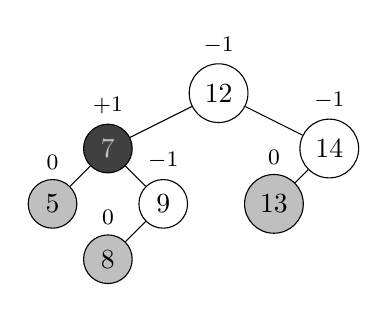
\begin{tikzpicture}[main/.style = {draw, circle}, level distance=2em,
		level 1/.style={sibling distance=8em},
		level 2/.style={sibling distance=4em}]
	\node[main, label={\footnotesize $-1$},fill=white] (root) {12}
    child { node[main, label={\footnotesize $+1$}, fill=darkgray] (l) {\color{lightgray} 7} 
    		child { node[main, label={\footnotesize $0$}, fill=lightgray] (ll) {5} }
    		child { node[main, label={\footnotesize $-1$},fill=white] (lr) {9} 
    			child {
    				node[main, label={\footnotesize $0$},fill=lightgray] (lrl) {8}
    			}
    			child[missing]{}
    		}
    	}
    child { node[main, label={\footnotesize $-1$},fill=white] (r) {14} 
    		child{ node[main,label={\footnotesize $0$},fill=lightgray] (rl) {13}}
    		child[missing]{}
    };
	\end{tikzpicture}
	\qquad
	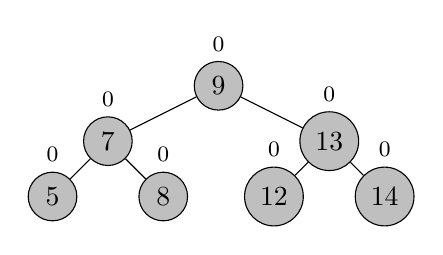
\begin{tikzpicture}[main/.style = {draw, circle}, level distance=2em,
		level 1/.style={sibling distance=8em},
		level 2/.style={sibling distance=4em}]
	\node[main, label={\footnotesize $0$},fill=lightgray] (root) {9}
    child { node[main, label={\footnotesize $0$}, fill=lightgray] (l) {7} 
    		child { node[main, label={\footnotesize $0$}, fill=lightgray] (ll) {5}}
    		child { node[main, label={\footnotesize $0$},fill=lightgray] (lr) {8} }
    	}
    child { node[main, label={\footnotesize $0$},fill=lightgray] (r) {13} 
    		child{ node[main,label={\footnotesize $0$},fill=lightgray] (rl) {12}}
    		child{ node[main,label={\footnotesize $0$},fill=lightgray] (rr) {14} }
    };
	\end{tikzpicture}
	\end{center}
	\end{exampleblock}
	Balance factors are listed above each respective node
\end{frame}

\begin{frame}{Standard AVL Tree: Examples}
	\begin{alertblock}{Invalid AVL Tree}
	\begin{center}
	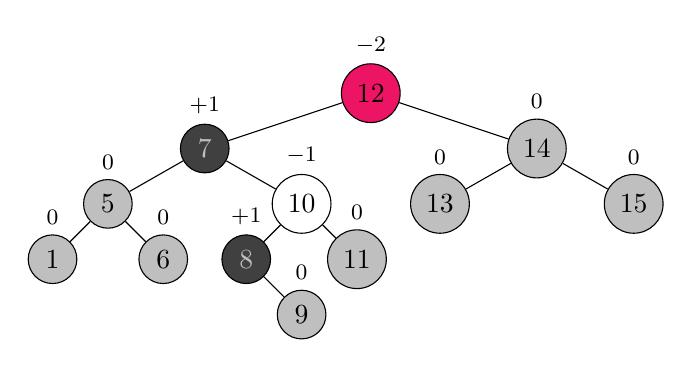
\begin{tikzpicture}[main/.style = {draw, circle}, level distance=2em,
		level 1/.style={sibling distance=12em},
		level 2/.style={sibling distance=7em},
		level 3/.style={sibling distance=4em}]
	\node[main, label={\footnotesize $-2$},fill=WildStrawberry] (root) {12}
    child { node[main, label={\footnotesize $+1$}, fill=darkgray] (l) {\color{lightgray} 7} 
    		child { node[main, label={\footnotesize $0$}, fill=lightgray] (ll) {5}
    			child{ node[main, label={\footnotesize $0$}, fill=lightgray] (lll) {1} }
    			child{ node[main, label={\footnotesize $0$}, fill=lightgray] (llr) {6} }
    		}
    		child { node[main, label={\footnotesize $-1$},fill=white] (lr) {10} 
    			child { node[main, label={\footnotesize $+1$},fill=darkgray] (lrl) {\color{lightgray}8}
    				child[missing]{}
    				child{ node[main, label={\footnotesize $0$}, fill=lightgray] (lrlr) {9}}
    			}
    			child {
    				node[main, label={\footnotesize $0$}, fill=lightgray] (lrr) {11}
    			}
    		}
    	}
    child { node[main, label={\footnotesize $0$},fill=lightgray] (r) {14} 
    		child{ node[main,label={\footnotesize $0$},fill=lightgray] (rl) {13}}
    		child{ node[main, label={\footnotesize $0$}, fill=lightgray] (rr) {15}}
    };
	\end{tikzpicture}
	\end{center}
	\end{alertblock}
\end{frame}

\begin{frame}{Standard AVL Tree: Cases}
Balancing for a standard AVL tree can be broken down into a few cases
\pause
\begin{itemize}
\item Left Left: Node $X$ has $\fun{BF}(X) < -1$,  $\fun{BF}(\fun{Left}(X)) \le 0$
\item Left Right: Node $X$ has $\fun{BF}(X) < -1$, $\fun{BF}(\fun{Left}(X)) > 0$
\item Right Left: Node $X$ has $\fun{BF}(X) > +1$, $\fun{BF}(\fun{Right}(X)) < 0$
\item Right Right: Node $X$ has $\fun{BF}(X) > +1$, $\fun{BF}(\fun{Right}(X)) \ge 0$
\item No-op: Node $X$ has $-1 \le \fun{BF}(X) \le +1$
\end{itemize}
\pause
Note: if $\fun{BF}(X) > 1 \vee \fun{BF}(X) < -1$, then we can guarantee that $X$ has at least a child and a grandchild.
\end{frame}

\begin{frame}{Standard AVL Tree: Case Left Left}
\begin{center}
	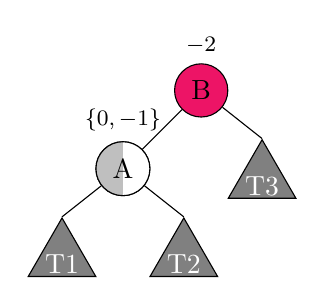
\begin{tikzpicture}[main/.style = {draw, circle}, leaves/.style = {draw, isosceles triangle, inner sep=1pt, shape border rotate=90,anchor=center,isosceles triangle apex angle=60}, node distance=4em and 1em]
	\node[main, label={\footnotesize $-2$},fill=WildStrawberry] (root) {B};
	\node[leaves,fill=gray, below right of=root, anchor=right side] (r) {\color{white}T3};
	\node[main,label={\footnotesize $\{0, -1\}$}, below left of=root] (l) {A};
	\path let \p1=($(l.west)-(l.east)$), 
			\n1 = {veclen(\p1)-\pgflinewidth},
			\n2 = {\n1/2}
	in  node (s2) [circle, fill=white, minimum size=\n1,at={(l.center)}] {}
		node [semicircle, fill=lightgray, 
                inner sep=0pt, outer sep=0pt, minimum size=\n2,
                anchor=south,
                at={(s2.center)}, rotate=90] {};
                
	\node[leaves, fill=gray, below left of=l, anchor=left side] (ll) {\color{white}T1};
	\node[leaves,fill=gray,below right of=l,anchor=right side] (lr) {\color{white}T2};
	\node[main,below left of=root] (lNew) {A};
	\draw (root) -- (r.apex);
 	\draw (root) -- (l);
 	\draw (l) -- (ll.apex);
 	\draw (l) -- (lr.apex);
	\end{tikzpicture}
\end{center}
\begin{itemize}
\pause \item $\textsf{B}$ is the first unbalanced node we encounter after an operation
\pause \item Only operations on the decedents of $\textsf{B}$ can cause $\textsf{B}$ to become imbalanced
\pause \item Thus, we will always encounter highest depth imbalanced node by traversing to the root
\pause \item Thus $\textsf{T1}$, $\textsf{T2}$, $\textsf{T3}$ must be balanced
\end{itemize}
\end{frame}

\newcommand{\leftleftdiagram}{
	\begin{center}
		\begin{tabular}{c c c}
			\begin{tabular}{l}
				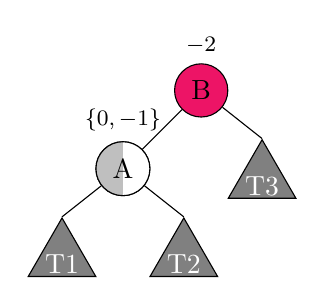
\begin{tikzpicture}[main/.style = {draw, circle}, leaves/.style = {draw, isosceles triangle, inner sep=1pt, shape border rotate=90,anchor=center,isosceles triangle apex angle=60}, node distance=4em and 1em]
					\node[main, label={\footnotesize $-2$},fill=WildStrawberry] (root) {B};
					\node[leaves,fill=gray, below right of=root, anchor=right side] (r) {\color{white}T3};
					\node[main,label={\footnotesize $\{0, -1\}$}, below left of=root] (l) {A};
					\path let \p1=($(l.west)-(l.east)$), 
					\n1 = {veclen(\p1)-\pgflinewidth},
					\n2 = {\n1/2}
					in  node (s2) [circle, fill=white, minimum size=\n1,at={(l.center)}] {}
					node [semicircle, fill=lightgray, 
					inner sep=0pt, outer sep=0pt, minimum size=\n2,
					anchor=south,
					at={(s2.center)}, rotate=90] {};
					
					\node[leaves, fill=gray, below left of=l, anchor=left side] (ll) {\color{white}T1};
					\node[leaves,fill=gray,below right of=l,anchor=right side] (lr) {\color{white}T2};
					\node[main,below left of=root] (lNew) {A};
					\draw (root) -- (r.apex);
					\draw (root) -- (l);
					\draw (l) -- (ll.apex);
					\draw (l) -- (lr.apex);
				\end{tikzpicture} 
			\end{tabular} &
			\begin{tabular}{l}
				$\boldsymbol{\longrightarrow}$ 
			\end{tabular} &
			\begin{tabular}{l}
				\begin{tikzpicture}[main/.style = {draw, circle}, leaves/.style = {draw, isosceles triangle, inner sep=1pt, shape border rotate=90,anchor=center,isosceles triangle apex angle=60}, node distance=4em and 1em]
					\node[main, label={\footnotesize $\{+1, 0\}$}] (root) {A};
					\node[main,label={\footnotesize $\{-1, 0\}$}, below right of=root] (r) {B};
					\path let \p1=($(l.west)-(l.east)$), 
					\n1 = {veclen(\p1)-\pgflinewidth},
					\n2 = {\n1/2}
					in  node (s2) [circle, fill=lightgray, minimum size=\n1,at={(r.center)}] {}
					node [semicircle, fill=white, 
					inner sep=0pt, outer sep=0pt, minimum size=\n2,
					anchor=south,
					at={(s2.center)}, rotate=90] {};
					\path let \p1=($(root.west)-(root.east)$), 
					\n1 = {veclen(\p1)-\pgflinewidth},
					\n2 = {\n1/2}
					in  node (s2) [circle, fill=lightgray, minimum size=\n1,at={(root.center)}] {}
					node [semicircle, fill=darkgray, 
					inner sep=0pt, outer sep=0pt, minimum size=\n2,
					anchor=south,
					at={(s2.center)}, rotate=90] {};
					\node[leaves,fill=gray, below right of=r, anchor=right side] (rr) {\color{white}T3};
					\node[leaves, fill=gray, below left of=root, anchor=left side] (l) {\color{white}T1};
					\node[leaves,fill=gray,below left of=r,anchor=left side] (rl) {\color{white}T2};
					\node[main,below right of=root] (rNew) {B};
					\node[main,at={(root.center)}] (rootNew) {\color{white}A};
					\draw (root) -- (r);
					\draw (root) -- (l.apex);
					\draw (r) -- (rr.apex);
					\draw (r) -- (rl.apex);
				\end{tikzpicture}
			\end{tabular}
		\end{tabular}
	\end{center}
}

\begin{frame}{Standard AVL Tree: Case Left Left}
	\leftleftdiagram
	\begin{itemize}
		\pause \item Rotate $\textsf{B}$ to the right (moving it down)
		\pause \item Resulting balance factors $\fun{BF'}(A)$ and $\fun{BF'}(B)$ dependent on initial balance factor $\fun{BF}(A)$ as indicated by the colors
		\pause \item Only two cases $\fun{BF}(A) \in \{0, -1\}$
	\end{itemize}
\end{frame}

\begin{frame}{Standard AVL Tree: Case Left Left}
	\leftleftdiagram
	\begin{itemize}
		\item Let $\fun{Height}(\textsf{T1}) = t_1, \fun{Height}(\textsf{T2}) = t_2, \fun{Height}(\textsf{T3}) = t_3$
		\pause \item We know $\fun{BF}(\textsf{A}) = t_2 - t_1 \in \{0, -1\}$, $\fun{BF}(\textsf{B}) = t_3 - (\fun{max}(t_1, t_2) + 1) = -2$
		\pause \item We know $t_1 \ge t_2 \wedge t_3 < t_1$. Thus $\fun{BF}(\textsf{B}) = t_3 - t_1 - 1 = -2$
	\end{itemize}
\end{frame}

%\end{frame}
\begin{frame}{Standard AVL Tree: Case Left Left}
	\leftleftdiagram
	\begin{itemize}
		\item We know $\fun{BF'}(\textsf{B}) = t_3 - t_2$ and $t_3 - t_1 = -1$
		\pause
		\begin{itemize}
			\item $t_2 = t_1 \implies \fun{BF'}(\textsf{B}) = t_3 - t_1 = -1$
			\item $t_2 = t_1 - 1 \implies \fun{BF'}(\textsf{B}) = t_3 - t_1 + 1 = 0$
		\end{itemize}
		\pause \item We know $\fun{BF'}(\textsf{A}) = \fun{max}(t_3, t_2) + 1 - t_1$ and $t_1 > t_3$
		\pause 
		\begin{itemize}
			\item $t_2 = t_1 \implies \fun{BF'}(\textsf{A}) = \fun{max}(t_3, t_1) + 1 - t_1 = 1$
			\item $t_2 = t_1 - 1 \implies \fun{BF'}(\textsf{A}) = \fun{max}(t_3, t_1 - 1) + 1 - t_1 = 0$
		\end{itemize}
	\end{itemize}
\end{frame}


\begin{frame}{Standard AVL Tree: Case Left Right}
\begin{center}
	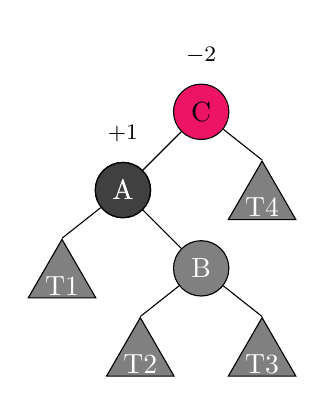
\begin{tikzpicture}[main/.style = {draw, circle}, leaves/.style = {draw, isosceles triangle, inner sep=1pt, shape border rotate=90,anchor=center,isosceles triangle apex angle=60}, node distance=4em and 1em, minimum size=2em]
		\node[main, label={\footnotesize $-2$},fill=WildStrawberry] (root) {C};
		\node[leaves,fill=gray, below right of=root, anchor=right side] (r) {\color{white}T4};
		\node[main,fill=darkgray, label={\footnotesize $+1$}, below left of=root] (l) {\color{white}A};
		
		\node[leaves, fill=gray, below left of=l, anchor=left side] (ll) {\color{white}T1};
		\node[main, fill=gray, below right of=l] (lr) {\color{white}B};
		\node[leaves,fill=gray,below right of=lr,anchor=right side] (lrr) {\color{white}T3};
		\node[leaves,fill=gray,below left of=lr,anchor=left side] (lrl) {\color{white}T2};
		\node[main,below left of=root] (lNew) {\color{white} A};
		\draw (root) -- (r.apex);
		\draw (root) -- (l);
		\draw (l) -- (ll.apex);
		\draw (l) -- (lr);
		\draw (lr) -- (lrl.apex);
		\draw (lr) -- (lrr.apex);
	\end{tikzpicture}
	\pause
	
	$\textsf{B}$, $\textsf{T1}$, $\textsf{T2}$, $\textsf{T3}$, and $\textsf{T4}$ are all balanced
\end{center}
\end{frame}
\newcommand{\leftrightdiagram}{
	\begin{center}
		\begin{tabular}{c c c}
			\begin{tabular}{l}
				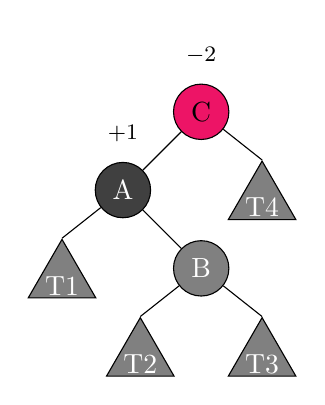
\begin{tikzpicture}[main/.style = {draw, circle}, leaves/.style = {draw, isosceles triangle, inner sep=1pt, shape border rotate=90,anchor=center,isosceles triangle apex angle=60}, node distance=4em and 1em, minimum size=2em]
					\node[main, label={\footnotesize $-2$},fill=WildStrawberry] (root) {C};
					\node[leaves,fill=gray, below right of=root, anchor=right side] (r) {\color{white}T4};
					\node[main,fill=darkgray,label={\footnotesize $+1$}, below left of=root] (l) {\color{white}A};
					\node[leaves, fill=gray, below left of=l, anchor=left side] (ll) {\color{white}T1};
					\node[main, fill=gray, below right of=l] (lr) {\color{white}B};
					\node[leaves,fill=gray,below right of=lr,anchor=right side] (lrr) {\color{white}T3};
					\node[leaves,fill=gray,below left of=lr,anchor=left side] (lrl) {\color{white}T2};
					\draw (root) -- (r.apex);
					\draw (root) -- (l);
					\draw (l) -- (ll.apex);
					\draw (l) -- (lr);
					\draw (lr) -- (lrl.apex);
					\draw (lr) -- (lrr.apex);
				\end{tikzpicture}  
			\end{tabular} &
			\begin{tabular}{l}
				$\boldsymbol{\longrightarrow}$  
			\end{tabular} &
			\begin{tabular}{l}
				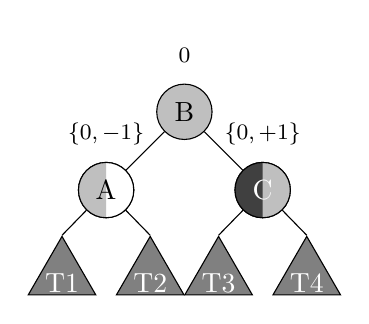
\begin{tikzpicture}[main/.style = {draw, circle}, leaves/.style = {draw, isosceles triangle, inner sep=1pt, shape border rotate=90,anchor=center,isosceles triangle apex angle=60}, node distance=4em, minimum size=2em]
					\node[main, label={\footnotesize $0$},fill=lightgray] (root) {B};
					\node[main,label={\footnotesize $\{0, -1\}$}, below left of=root] (l) {A};
					\path let \p1=($(l.west)-(l.east)$), 
					\n1 = {veclen(\p1)-\pgflinewidth},
					\n2 = {\n1/2}
					in  node (s2) [circle, fill=white, minimum size=\n1,at={(l.center)}] {}
					node [semicircle, fill=lightgray, 
					inner sep=0pt, outer sep=0pt, minimum size=\n2,
					anchor=south,
					at={(s2.center)}, rotate=90] {};
					
					\node[main, label={\footnotesize $\{0, +1\}$}, fill=gray, below right of=root] (r) {C};
					\path let \p1=($(r.west)-(r.east)$), 
					\n1 = {veclen(\p1)-\pgflinewidth},
					\n2 = {\n1/2}
					in  node (sr2) [circle, fill=lightgray, minimum size=\n1,at={(r.center)}] {}
					node [semicircle, fill=darkgray, 
					inner sep=0pt, outer sep=0pt, minimum size=\n2,
					anchor=south,
					at={(sr2.center)}, rotate=90] {};
					\node[leaves, fill=gray, below left=2em and 1.5em of l, anchor=left side] (ll) {\color{white}T1};
					\node[leaves,fill=gray,below right=2em and 1.5em of l,anchor=right side] (lr) {\color{white}T2};
					\node[leaves,fill=gray, below right=2em and 1.5em of r, anchor=right side] (rr) {\color{white}T4};
					\node[leaves,fill=gray, below left=2em and 1.5em of r,anchor=left side] (rl) {\color{white}T3};
	
					\node[main,below left of=root] (lNew) {A};
					\node[main,below right of=root] (rNew) {\color{white}C};
					\draw (root) -- (r);
					\draw (root) -- (l);
					\draw (l) -- (ll.apex);
					\draw (l) -- (lr.apex);
					\draw (r) -- (rl.apex);
					\draw (r) -- (rr.apex);
					% T1: h
					% T2: i 
					% T3: j
					% T4: k
					% max(i, j) = h, max(i, j)+ 1 = h ==> max(i, j) <= h
					% BF(B) = j - i
					% BF(A) = max(i, j) + 1 - h  = {0, 1} 
					% BF(C) = k - (max(h, max(i, j) + 1) + 1) = -2
					% max(i, j) + 1 - h >= 0, max(i, j) + 1 >= h
					% BF(C) = k - (max(i, j) + 2) = -2
					%     k - max(i, j) - 2 = -2
					%     k = max(i, j)
					
					
					% -1 <= j - i <= 1
					% 0 <= j - i + 1 <= 2
					% BF'(A) = i - h
					% BF'(C) = k - j
					%    max(i, j) - j
					%    	if  j >= i, then 0
					%       if j < i then -BF(B)
					% BF'(B) = max(k, j) - max(i, h)
					
					% a = 1, b = -1
					%    h = i
					%    j + 1 = i
					%    k - (i + 2) = -2; k = i; 
					%    BF'(A) = 0
					%    BF'(C) =  j + 1 - j = 1
					%    BF'(B) = k - i = 0
					
					% a = 1, b = 0
					%    h = i
					%    j = i
					%    k - (i+2) = -2; k = i
					%    BF'(A) = 0
					%    BF'(C) = 0
					%    BF'(B) = max(j - 1, j) - max(j, j) = 0

					% a = 1, b = 1
					%     j - i = 1; j = i + 1
					%     j + 1 - h = 1; j - h = 0
					%    k - (j + 2) = -2; k = j
					%    BF'(A) = i - (i + 1) = -1
					%    BF'(C) = k - j = 0
					%    BF'(B) = 0				
					
					
					% b = -1 -> BF(C) = 1
					% b = {0, 1} -> BF(C) = 0
					% b = 1 -> BF(A) = -1
					% b = {0, -1} -> BF(A) = 0
					% BF(C) = if BF(B) >= 0 then 0 else 1
					% BF(A) = if BF(B) <= 0 then 0 else -1	
				\end{tikzpicture}
			\end{tabular}
		\end{tabular}
	\end{center}
}
\begin{frame}{Standard AVL Tree: Case Left Right}
	\leftrightdiagram
	\begin{itemize}
		\pause \item Let $\fun{Height}(T1) = t_1, \cdots, \fun{Height}(T4) = t_4$ 
		\pause \item We can see/easily prove $t_1 = \fun{max}(t_2, t_3) = t_4$
		\pause \item Thus $\fun{BF'}(B) = \fun{max}(t_3, t_4) - \fun{max}(t_1, t_2) = 0$
	\end{itemize}
\end{frame}
\begin{frame}[noframenumbering]{Standard AVL Tree: Case Left Right}
	\leftrightdiagram
	\begin{itemize}
		\item We know $\fun{BF'}(A) = t_2 - t_1$
		\pause \item If $\fun{BF}(B) \le 0$ then $\fun{max}(t_2, t_3) = t_2$
			\begin{itemize}
				\item So $t_1 = t_2 = t_4$
				\item Thus $\fun{BF'}(A) = 0$
			\end{itemize} 
		\pause \item If $\fun{BF}(B) > 0$ then $t_3 - t_2 = 1$ since $B$ is balanced
			\begin{itemize}
				\item So $t_1 = \fun{max}(t_2, t_3) = \fun{max}(t_2, t_2 + 1) = t_2 + 1$
				\item Thus $\fun{BF'}(A) = t_2 - t_1 = -1$
			\end{itemize}
	\end{itemize}
\end{frame}
\begin{frame}[noframenumbering]{Standard AVL Tree: Case Left Right}
	\leftrightdiagram
	\begin{itemize}
		\item We know $\fun{BF'}(C) = t_4 - t_3$
		\pause \item If $\fun{BF}(B) \ge 0$ then $\fun{max}(t_2, t_3) = t_3$
		\begin{itemize}
			\item So $t_1 = t_3 = t_4$
			\item Thus $\fun{BF'}(C) = 0$
		\end{itemize} 
		\pause \item If $\fun{BF}(B) < 0$ then $t_3 - t_2 = -1$ since $B$ is balanced
		\begin{itemize}
			\item So $t_4 = \fun{max}(t_2, t_3) = \fun{max}(t_3 + 1, t_3) = t_3 + 1$
			\item Thus $\fun{BF'}(C) = t_4 - t_3 = +1$
		\end{itemize}
	\end{itemize}
\end{frame}
\begin{frame}[noframenumbering]{Standard AVL Tree: Case Left Right}
	\leftrightdiagram
	\begin{center}
	\textbf{Summary}
	
	\begin{tabular} {r l}
		$\fun{BF'}(A)$ &$= -\fun{max}(\fun{BF}(B), 0)$ \\ 
		$\fun{BF'}(B)$ &$= 0$\\
		$\fun{BF'}(C)$ &$= -\fun{min}(\fun{BF}(B), 0)$
	\end{tabular}
	\end{center}
\end{frame}

\begin{frame}{$k$-AVL Tree}
	Same as AVL tree,  except property (2) is changed to
	\begin{equation}\label{kavlProperty}\tag{2}
	\fun{BF}(X) \in \{x \in \mathbb{N} \mid -k \le x \le k\}
	\end{equation}
	\begin{itemize}
	\pause \item In fact, the $1$-AVL tree is equivalent to our standard AVL tree
	\pause \item $k$ does not need to be fixed, can be a dependent on number of nodes $n$
	\pause \item $n$-AVL tree is equivalent to a non-balancing BST 
	\end{itemize}
\end{frame}

\begin{frame}{$k$-AVL Tree}
	\begin{block}{The simple solution}
		Store the height on each node, then check balance factors by subtraction
	\end{block}
	\pause % Automatically creates a new "page" split between the above and above + below
	\begin{alertblock}{The problem}
		Have to traverse to the root on every operation to set height
	\end{alertblock}
	\pause % Automatically creates a new "page" split between the above and above + below
	\begin{exampleblock}{Question}
		Is it possible to only store balance factors at each node and not have to traverse to the root?
	\end{exampleblock}
\end{frame}

\begin{frame}{$k$-AVL Tree: Cases}
	
\end{frame}

\begin{frame}[plain]{Plain Slide}
	This is a slide with the plain style and it is numbered.
\end{frame}

%------------------------------------------------

\begin{frame}[t]
	This slide has an empty title and is aligned to top.
\end{frame}

%------------------------------------------------

\begin{frame}[noframenumbering]{No Slide Numbering}
	This slide is not numbered and is citing reference \cite{knuth74}.
\end{frame}

%------------------------------------------------

\begin{frame}{Typesetting and Math}
	The packages \texttt{inputenc} and \texttt{FiraSans}\footnote{\url{https://fonts.google.com/specimen/Fira+Sans}}\textsuperscript{,}\footnote{\url{http://mozilla.github.io/Fira/}} are used to properly set the main fonts.
	\vfill
	This theme provides styling commands to typeset \emph{emphasized}, \alert{alerted}, \textbf{bold}, \textcolor{example}{example text}, \dots
	\vfill
	\texttt{FiraSans} also provides support for mathematical symbols:
	\begin{equation*}
		e^{i\pi} + 1 = 0.
	\end{equation*}
\end{frame}

%----------------------------------------------------------------------------------------
%	 SECTION 2
%----------------------------------------------------------------------------------------

\section{Section 2}

%------------------------------------------------

\begin{frame}{Blocks}
	These blocks are part of 1 slide, to be displayed consecutively.
	\begin{block}{Block}
		Text.
	\end{block}
	\pause % Automatically creates a new "page" split between the above and above + below
	\begin{alertblock}{Alert block}
		Alert \alert{text}.
	\end{alertblock}
	\pause % Automatically creates a new "page" split between the above and above + below
	\begin{exampleblock}{Example block}
		Example \textcolor{example}{text}.
	\end{exampleblock}
\end{frame}

%------------------------------------------------

\begin{frame}{Columns}
	\begin{columns}
		\column{0.5\textwidth}
			This text appears in the left column and wraps neatly with a margin between columns.
		\pause
		\column{0.5\textwidth}
			\includegraphics[width=\linewidth]{Images/placeholder.jpg}
	\end{columns}
\end{frame}

%------------------------------------------------

\begin{frame}{Lists}
	\begin{columns}[T, onlytextwidth] % T for top align, onlytextwidth to suppress the margin between columns
		\column{0.33\textwidth}
			Items:
			\begin{itemize}
				\item Item 1
				\begin{itemize}
					\item Subitem 1.1
					\item Subitem 1.2
				\end{itemize}
				\item Item 2
				\item Item 3
			\end{itemize}
		
		\column{0.33\textwidth}
			Enumerations:
			\begin{enumerate}
				\item First
				\item Second
				\begin{enumerate}
					\item Sub-first
					\item Sub-second
				\end{enumerate}
				\item Third
			\end{enumerate}
		
		\column{0.33\textwidth}
			Descriptions:
			\begin{description}
				\item[First] Yes.
				\item[Second] No.
			\end{description}
	\end{columns}
\end{frame}

%------------------------------------------------

\begin{frame}{Table}
	\begin{table}
		\centering % Centre the table on the slide
		\begin{tabular}{l c}
			\toprule
			Discipline & Avg. Salary \\
			\toprule
			\textbf{Engineering} & \textbf{\$66,521} \\
			Computer Sciences & \$60,005\\
			Mathematics and Sciences & \$61,867\\
			Business & \$56,720\\
			Humanities \& Social Sciences & \$56,669\\
			Agriculture and Natural Resources & \$53,565\\
			Communications & \$51,448\\
			\midrule
			\textbf{Average for All Disciplines} & \textbf{\$58,114}\\
			\bottomrule
		\end{tabular}
	\caption{Table caption}
	\end{table}
\end{frame}

%------------------------------------------------

\begin{frame}[focus]
	Thanks for using \textbf{Focus}!
\end{frame}

%----------------------------------------------------------------------------------------
%	 CLOSING/SUPPLEMENTARY SLIDES
%----------------------------------------------------------------------------------------

\appendix

\begin{frame}{References}
	\nocite{*} % Display all references regardless of if they were cited
	\bibliography{example.bib}
	\bibliographystyle{plain}
\end{frame}

%------------------------------------------------

\begin{frame}{Backup Slide}
	This is a backup slide, useful to include additional materials to answer questions from the audience.
	\vfill
	The package \texttt{appendixnumberbeamer} is used to refrain from numbering appendix slides.
\end{frame}

%----------------------------------------------------------------------------------------

\end{document}
